\documentclass[english]{article}

\usepackage[nodayofweek]{datetime}

\title{\textbf{Title} \\subtitle}
\author{Zhao Lyu}
%\date{2018-01-15}%change \today


\usepackage{amsmath, mathtools, amsfonts,amssymb,flexisym,enumitem,grffile,graphicx,tikz,subcaption,titling}
\usepackage{tikz}
\usepackage{tkz-euclide}
\usetkzobj{all}
\usepackage{wrapfig,blindtext,babel,calc}
%\usetikzlibrary{intersections,calc}
\usepackage{setspace}
\setlist[enumerate]{itemsep=0mm}
\graphicspath{{/home/user/Project199/Figures}}

\usepackage{amsthm}
\newtheorem*{definition*}{Definition}
\newtheorem{definition}{Definition}
\newtheorem{theorem}{Theorem}
\newtheorem*{theorem*}{Theorem}
\newtheorem*{lemma*}{Lemma}
\newtheorem{lemma}{Lemma}
\newtheorem*{claim*}{Claim}
\newtheorem{claim}{Claim}

\newcommand{\vol}{\operatorname{vol}}
\newcommand{\diam}{\operatorname{diam}}


\begin{document}

  \doublespacing %use setspace package
  %\maketitle{Refinement Strategy in 2 Dimension}
  \title{Refinement Strategy in 2 Dimension}
  \maketitle
  \singlespacing

  \newpage %separate title and contents
  \pagenumbering{gobble}
  \tableofcontents
  \newpage
  \pagenumbering{arabic}

  %\section{Introduction}
  %introduction
  %\newpage

  \section{Basic Definition}
    We first recall definitions of linear transformation and translation, and further introduce affine transformations, which we will use to prove stability of uniform mesh refinement and bisection in sections later. Then we introduce basic notions which we will use to present mesh refinement and show how they would work out.

       \subsection{Translation, Linear Transformation and Affine Transformation}
      
      We define several classes of transformations that we frequently use.
      %sets\\
      linear, translation, affine transformation\\
      
      \begin{definition*}
        %$\textbf{Translation}$\\
         Let $\textbf{v}$ be a fixed vector, a $\textbf{translation}$ ${T}_v$ on a figure applies as ${T}_v (\textbf{p}) = \textbf{p} + \textbf{v}$, for a vector $\textbf{p}$ in the figure which we translate.
      \end{definition*}
      A $\textit{translation}$ moves every point of a figure or space by the same distance in the same direction. A translation ${T}$ can be represented by an addition of a constant vector to every point.\\


      \begin{definition*}
      %\paragraph{Linear transformation}
      Let ${V}$ and ${W}$ be vector spaces over the same field $\textbf{K}$. We say a function $\mathit{f}: {V} \rightarrow {W}$ is $\textbf{linear transformation}$ if the following is satisfied:\\
      \begin{align*}
      \mathit{f}(\textbf{u} + \textbf{v}) &= \mathit{f}(\textbf{u}) + \mathit{f}(\textbf{v}) \qquad \forall \textbf{u}, \textbf{v} \in{V},\\
      \mathit{f}(c\textbf{u}) &= c\mathit{f}(\textbf{u}), \qquad \forall \textbf{u} \in{V}, ~c\in\textbf{K}.
      \end{align*}
      \end{definition*}
      In other words, a linear transformation is a mapping between two vector spaces which preserves the operations of addition and scalar multiplication. Moreover, if ${V}$ and ${W}$ are finite dimensional, we can represent the linear transformation ${f}$ by a matrix ${M}$. For example, if ${M}$ is an ${m} \times {n}$ matrix, then ${f}$ is a linear transformation from $\mathbf{R}^n$ to $\mathbf{R}^m$. \\


      \begin{definition*}
      %\paragraph{Affine Transformation}
      An $\textbf{affine transformation}$ from $\mathbb{R}^n$ to $\mathbb{R}^n$ is of the form\\
      \begin{equation*}
      {F}(x) = {Ax} + {v}, \qquad {x}\in\mathbb{R}^n,
      \end{equation*}
      where ${A}\in\mathbb{R}^{n\times n}$ is a linear transformation, and  ${v}\in\mathbb{R}^n$ is a translation vector.\\
      \end{definition*}
      Affine transformation preserves points, lines and planes, but need not preserve point zero in a linear space in contrast to linear transformation. So we see that translation and linear transformation is affine, but the opposite is not true.\\
      %\indent
      The inverse mapping is only defined if $A^{-1}$ exists, and we define the inverse mapping $F^{-1} = {x} \mapsto {A}^{-1}({x} - {v})$ is also an affine transformation. Affine transformation helps carry results from one simplex to another simplex in our discussion, and more details are covered after introducing ${Simplices}$ and ${Triangulations}$ in the next section.



        \subsection{Simplices}
    \noindent
    \begin{definition*}
    A $\textbf{k-simplex T}$ $\in{R}^n$ is a ${k-}$dimensional convex hull of ${k}$ + 1 vertices ${x}_0, \cdots, {x}_k \in \mathbb{R}^n$, which are affinely independent.\\
    \begin{equation*}
    \begin{split}
    {T} & = [{x}_0, \cdots, {x}_k ]\\
    & := \left\{{x} = \sum\limits_{i=0}^k \lambda_i {x}_i \Bigm| \sum\limits_{i=0}^k \lambda_i = 1 ~and~ 0 \leqslant \lambda_i \leqslant 1, 0 \leqslant i \leqslant k \right\}\\
    & := \left\{\lambda_0{x}_0 + \cdots + \lambda_k{x}_k \Bigm| \sum\limits_{i=0}^k \lambda_i = 1 ~and~ 0 \leqslant \lambda_i \leqslant 1, 0 \leqslant i \leqslant k \right\}.
    \end{split}
    \end{equation*}
    \end{definition*}
    If ${k} = n$, we can call ${k-simplex}$ without addressing the dimension. 2-simplices are also called ${triangle}$, and 3-simplices are called ${tetrahedra}$.

    \begin{definition*}
    %\paragraph{Subsimplices}
    An ${l-}$simplex ${S} = [{y}_0, \cdots, {y}_l]$ is called an $\textbf{l-subsimplex}$ of ${k-}$simplex ${T} = [{x}_0, \cdots, {x}_k]$, if indices $0 \leqslant {i}_0 \leqslant \cdots\leqslant{i}_l \leqslant k$ with ${y}_i = {x}_i$, for $0 \leqslant l \leqslant k \leqslant n$.
    \end{definition*}
    Since there are $k+1$ vertices in ${k-}$simplex ${T}$, and $l+1$ vertices in ${l-}$subsimplex ${S}$, the number of ${l-}$subsimplex of ${k-}$simplex is $\binom{k+1}{l+1}$.


    %\paragraph{Simplices Equality}
    Consider simplices ${T} = [{x}_0, \cdots, {x}_k]$ and $\text{T\textprime} = [{y}_0, \cdots, {y}_k]$. We say these two simplices ${T}$ and ${T\textprime}$ are equal, i.e. ${T} = {T\textprime}$, if ${x}_i = {y}_i$ for $0 \leqslant i \leqslant k$. Note that the vertex ordering of simplex is fixed, so if two simplices ${T}$ and ${T\textprime}$ denote the same set but with different vertex ordering, they are not equal; instead, we say that ${T}$ coincides with ${T\textprime}$, i.e. ${T} \cong {T\textprime}$.

    \paragraph{Simplex under Affine Transformation}\mbox{}\\
    Instead of taking a single variable $x\in\mathbb{R}^n$ for affine transformation, we can take a subset S $\subset \mathbb{R}^n$, which contains $x\in\mathbb{R}^n$. Then the transformed set $S\textprime$ is
    \begin{equation*}
    S\textprime= {F}(x) = \left\{{F}(x) ~|~ x\in S \right\}.
    \end{equation*}
    Similarly, if we regard a k-dimensional simplex ${T} = [{x_0, \cdots, x_k}]$ as a subset $\in\mathbb{R}^n$, then the image of ${T}$ under affine transformation, denoted by $T\textprime$, is defined as
    \begin{equation*}
    \begin{split}
    {T}\textprime & = {F}({T}) = \left\{{F}(x_0), \cdots , {F}(x_k)\right\}.
    \end{split}
    \end{equation*}
    We can see that ${T}\textprime$ is still a k-dimensional simplex. Furthermore, we can define ${F}({T}) = {AT} + {v}$, where $T$ is k-dimensional simplex $\in\mathbb{R}^n$. We might be curious about the relationship between simplices ${T}$ and ${T}\textprime$. Since vertices of a simplex are in a specific given order, so different vertex ordering leads to different simplices. Therefore, there exists an unique affine transformation such that ${T} = {T}\textprime$. Another important property of simplices is congruence.

    \begin{definition*}
    Two simplices T, T' are defined to be congruent if they can be obtained from each other by rotation, mirroring, scaling, and translation, i.e. if there exists a scaling factor c $\in\mathbb{R}^{+}$, a translation vector $v\in\mathbb{R}^n$, and an orthogonal matrix $Q\in\mathbb{R}^{n\times n}$ such that
    \begin{equation*}
    T' = v + cQT
    \end{equation*}
    \end{definition*}
    \noindent
    When the two simplices $T, T'$ have same vertices but with different vertex ordering, we can translate it as $T' = F(T)$. Based on how we define the affine transformation, it's not hard to see that ${T} \cong {T}\textprime$. Then we say that ${T}$ and ${T}\textprime$ are in a same congruent class.
    \subsection{Shape Regularity Measure}\mbox{}\\
    $\textit{Shape measure}$ offers an objective mathematical measure on the overall quality of an Finite Element mesh, and this is helpful to explore the simplex regularity and to improve the quality of shapes of the elements. Different definitions are used for shape measure to present the quality of simplex, and we simply introduce the $\textit{geometric shape measure} ~\mu({T})$ of simplex ${T}$,  the one we use in this paper.

    \paragraph{Simplex Diameter and Volume}\mbox{}\\
    Let ${T} \in\mathbb{R}^n$ be a k-simplex where $k \leqslant n$, with vertices ${x}_0, \cdots, {x}_k \in\mathbb{R}^n$. We let diam$({T})^k$ denote the diameter of ${T}$, and we define
    \begin{equation*}
    %\operator???
    \operatorname{diam}({T})^k = \max_{0\leqslant i\leqslant j\leqslant k} \| x_i - x_j \|
    \end{equation*}
    In other words, diam$({T})^k$ is the longest distance between two vertices of ${T}$, which is equivalent to the length of the longest edge of ${T}$. If ${T}$ is a single vertex, then diam$({T}) = 0$.\\

    \noindent
    Let vol$^k$(${T}$) denote k-dimensional volume of ${T}$. We have
    \begin{equation*}
    \operatorname{vol^k} ({T}) = \frac{1}{k!}\cdot|\det(x_1-x_0, x_2-x_0,\cdots, x_k-x_0)|
    \end{equation*}
    \noindent
    If k = 0, then ${T}$ is a 0-dimensional simplex, i.e., a vertex. By convention we have vol$^0 ({T})$ = 1, the vol$^0$ of a single vertex is one.

    
    \paragraph{Shape Measure}\mbox{}\\
    Simplex diameter and volume are important to introduce shape measures. Here we define the {geometric shape measure} $\mu({{T}})$ of a simplex ${T}$ by
    \begin{equation*}
    \mu({{T}}) = \frac{\operatorname{diam}({T})^k}{\operatorname{vol^k}({T})}, \quad\operatorname{vol^k(T) \neq 0}
    \end{equation*}
    If vol$^k(T)$ = 0, then we define $\mu({{T}}) = \infty$.\\
    
    To understand this definition, we can translate $\mu({{T}})$ as a measurement of how different the two variables, i.e. diam$({T})^k$ and vol$^k({T})$, are. For example, for a 3-dimensional simplex, i.e. a triangle, shape measure helps measure how narrow the triangle is. In other words, it measures how small the smallest angle of the triangle is. [Is this $\vol~\diam$ ???]

    \paragraph{Stability of a Simplex}\mbox{}\\
    The reason why we need shape measure is to help understanding whether a simplex $T$ is non-degenerate, and to quantify how degenerate or non-degenerate. Let $T$ be a k-dimensional simplex in $\mathbb{R}^n$. We say that a simplex $T$ is degenerate if and only if $\mu({T}) = \infty$, i.e. $\vol_k(T) = 0$. 

    
    %???
    \begin{figure}
    \centering
    \begin{tikzpicture}
    \draw (0,0) -- (3,2) -- (5,0)-- (0,0);
    \draw (7,0) -- (10,1) -- (12,0)-- (7,0);
    %\path (1,1) coordinate (A) (2.5, 2.5) coordinate (B) (3, 1) coordinate (C)
    %\draw (A) -- (B) -- (C) -- cycle
    \end{tikzpicture}
    \caption{Good triangle(left) with smaller shape measure vs. Bad triangle(right) with larger shape measure}
    \label{Fig1}
    \end{figure}

    Observing two triangles in Figure 1, we actually want the interior angles of the simple $T$, i.e. triangles in this example, to be uniformly bounded from zero. Thus vol$_2(T)$ will never go to 0.
    While cutting a simplex into smaller pieces, we want to keep those pieces uniformly bounded and avoid degenerate simplices. \\

    \begin{lemma*}
    If $T, T'$ are congruent simplices, then $\mu(T) = \mu(T')$.
    \end{lemma*}
    \begin{proof}\mbox{}\\
    Since $T$ is congruent to $T'$, by definition, we have $T' = v + cQT$, where $c\in\mathbb{R}^{+}$ is scaling factor, $v\in\mathbb{R}^n$ is a translation vector and $Q\in O(n)$ is an orthogonal matrix. In fact, we will show that scalings, translations, orthogonal transformation do not influence the shape measure of a simplex. 
    
    To be specific, when scaling a simplex $T$ by a non zero factor $c\in\mathbb{R}^{+}$ to obtain $T'$, we have 
    \begin{align*}
     vol^k(T') &= \frac{1}{k!}\cdot|\det(cx_1-cx_0, cx_2-cx_0,\cdots, cx_k-cx_0)| \\
               &= \frac{c^k}{k!}\cdot|\det(x_1-x_0, x_2-x_0,\cdots, x_k-x_0)| = c\cdot vol^k(T).
    \end{align*}
    Since it scales over all vertices, $diam(T')^k = c^k\cdot diam(T)^k$. Therefore, we see
    \begin{align*}
    \mu(T') = \frac{diam(T')^k}{vol^k(T')} = \frac{c^k\cdot diam(T)^k}{c^k\cdot vol^k(T)} = \frac{diam(T)^k}{vol^k(T)} = \mu(T)
    \end{align*}

    Moreover, translation over simplex $T$ by a nonsingular vector $v$ to obtain $T'$ will not influence the shape measure as well. In detail, we have
    \begin{align*}
    diam(T')^k &= \max_{0\leqslant i\leqslant j\leqslant k} \|(x_i + v) - (x_j + v)\|\\ 
               &= \max_{0\leqslant i\leqslant j\leqslant k}\|x_i - x_j\| = diam(T)^k \\
    vol^k(T') &= \frac{1}{k!}\cdot|\det((x_1+v) - (x_0+v), (x_2+v)-(x_0+v),\cdots,(x_k+v)-(x_0+v))|\\
              &= \frac{1}{k!}\cdot|\det(x_1-x_0, x_2-x_0,\cdots, x_k-x_0)| = vol^k(T)\\
    \mu(T') &= \frac{diam(T')^k}{vol^k(T')} = \frac{diam(T)^k}{vol^k(T)} = \mu(T)
    \end{align*}

    Consider rotating and mirroring $T$ by an orthogonal matrix $Q$ to obtain $T'$. Since $Q$ is an orthogonal matrix, $Q^T = Q^{-1}$. Therefore, we have
    \begin{align*}
    diam(T')^k &= \max_{0\leqslant i\leqslant j\leqslant k} \|Qx_i - Qx_j\|\\
               &= \max_{0\leqslant i\leqslant j\leqslant k} \|x_i - x_j\| = diam(T)^k&&\\
    vol^k(T') = vol^k(Q\cdot T) &= \frac{1}{k!}\cdot |\det(Q(x_1-x_0), Q(x_2-x_0),\cdots, Q(x_k-x_0)|\\
                                &= \frac{1}{k!}\cdot|det(Q)|\cdot|\det(x_1-x_0, x_2-x_0, \cdots, x_k-x_0)|\\
                                &= \frac{1}{k!}\cdot|-1|\cdot|\det(x_1-x_0, x_2-x_0, \cdots, x_k-x_0)|\\
                                &= \frac{1}{k!}\cdot|\det(x_1-x_0, x_2-x_0, \cdots, x_k-x_0)| = vol^k(T)\\
    \text{Therefore, we have } \mu(T') &= \frac{diam(T')^k}{vol^k(T')} = \frac{diam(T)^k}{vol^k(T)} = \mu(T)
    \end{align*}
    Now we see that the shape measure is independent of scaling, translation, rotation or mirroring. Thus a simplex $T'$ which is obtained by these motions shares a same shape measure with $T$.
    \end{proof}
    % !TEX root = Prokect199.tex
\subsection{Simplicial Complex(OR Triangulation)}
    \begin{definition*}
    A $\textbf{simplicial complex} ~~\mathcal T$ in $\mathbb{R}^n$ is a finite set of simplices in $\mathbb{R}^n$ that satisfies the following conditions:
    \begin{enumerate}[label =\arabic*.]
      \item Any face of a simplex from $\mathcal{T}$ is also in $\mathcal{T}$.
      \item The intersection of any two simplices ${T}_1, {T}_2 \in \mathcal{T}$ is a face of both ${T}_1$ and  ${T}_2$.
    \end{enumerate}
    \begin{figure}[b]
    \centering
    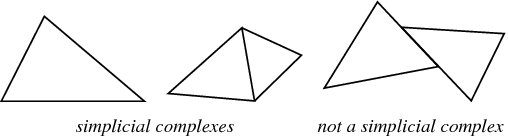
\includegraphics[width=60mm]{Figures/SimplicialComplex.png}
    \caption[Simplicial Complex Example and Counterexample]{Adopted from~\cite{WEBSITE:1}}%cite???
    \label{Fig2}
    \end{figure}
    \end{definition*}
    In other words, the first condition asks $\mathcal{T}$ to be closed under subsimplices, and the second condition asks that the intersection of any two simplices is either a common subsimplex or empty because the empty set is a face of every simplex. Examples in 2D are shown in Figure.1. \\
    \indent
    Any subset ${T\textprime}\in{T}$ that is itself a simplicial complex is called a $\textit{subcomplex}$ of ${T}$. A $\textit{simplicial k-complex} ~~\mathcal T$ is a simplicial complex where the largest dimension of any simplex in $\mathcal T$ is ${k}$. So a simplicial 2-complex must not contain tetrahedra or higher dimension simplices. The 0-complex of ${T}$ is called a $\textit{vertex set}$ of ${T}$. We can also think simplicial complex as a space with a triangulation, which is the division of a surface or a plane polygon into a set of 2-simplices. The constrains of triangulation will be discussed in ? section.\\

    \paragraph{Simplicial Complex under Affine Transformation}\mbox{}\\
    Extending further from simplex under affine transformation, now we know that simplicial complex is just a finite set of simplices. Therefore, we can define the Transformed Simplicial Complex $F(\mathcal{T})$ as follows
    \begin{equation*}
    F(\mathcal{T}) := \{F(T) \quad \vert \quad T\in \mathcal{T}\}
    \end{equation*}
    If $\mathcal{T}$ is consistent, then $F(\mathcal{T})$ is also consistent by inheriting this property from $\mathcal{T}$.

    \paragraph{Shape Measure of Simplicial Complex}\mbox{}\\
    We define shape measure of a simplex \(T \in\mathbb{R}^n$ as $\mu({{T}}) = \displaystyle \frac{\operatorname{diam}({T})^k}{\operatorname{vol^k}({T})}\). Now consider a simplicial complex $\mathcal{T}\in\mathbb{R}^n$, we define the geometric shape measure $\mu(\mathcal{T})$ as follows,
    \begin{equation*}
    \mu(\mathcal{T}) = \max_{T \in \mathcal{T}} \mu(T)
    \end{equation*}
    By definition, we see that the shape measure of a simplicial complex $\mathcal{T}$ is the supreme of the set of shape measures of all simplex $T\in\mathcal{T}$. If the largest shape measure of a simplex in this simplicial complex is bounded, then none of simplices in $\mathcal{T}$ is degenerate. In other words, if simplex $T_0 \in\mathcal{T}$ is non-degenerate, then simplicial complex $\mathcal{T}$ non-degenerate.
    [Correct?? Pf needed???]


  \section{Refinement Strategy in General}
    Refinement is a procedure of mesh modification in which we can divide a regular domain into smaller pieces under boundary constrains. This process can be applied recursively to simplify some differential equations by generating smaller pieces of the domain. Let us first introduce triangulation to help understand refinement on a simplex. Generally speaking, we can think triangulation as a subdivision of a plane into triangles. Definition below is a more formal way to take when extending to higher dimension.
    \begin{definition*}
    A triangulation of $\mathbb R^n$ is subdivision into n-dimensional simplices such that intersection of any two simplices is either empty or sharing a common face, and any face of a simplex is in the triangulation.
    \end{definition*}
    Indeed, we say that this triangulation is consistent as it is not simply subdividing of a space. Moreover, the triangulation defined here can be treated equivalently as simplicial complex as it is a finite set of simplices satisfying\\
    1. Any face of a simplex from a triangulation is also in the triangulation,\\
    2. The intersection of any two simplices ${T}_1, {T}_2 $ in a triangulation is a face of both ${T}_1$ and  ${T}_2$ or empty.
    (Denote triangulation same as simplicial complex $\mathcal{T}$)\\
    

    We can think a refinement of a simplex $T$ as a triangulation $\mathcal{T}$ which consists of smaller pieces of simplices of same type of the simplex $T$. Now consider a refinement of a simplicial complex. Let $\mathcal{T}$ and $\mathcal{T'}$ be two different simplicial complex covering a same domain $\Omega$. This means that the domain \(\Omega = \displaystyle \bigcup({T \vert T\in \mathcal{T}}) = \bigcup({T' \vert T\in \mathcal{T'}})\). We say that $\mathcal{T'}$ is a refinement of $\mathcal{T}$ if each simplex $T\in\mathcal{T}$ is in $\mathcal{T'}$ or the triangulation of $T$ is in $\mathcal{T'}$.

    As mentioned before, we may recursively apply a refinement strategy to help simplify some problems. By recursively taking refinement process from $\mathcal{T}_0$, we have a hierarchy triangulation $\mathcal{T}_k, k\in\mathbb{N}$, where $\mathcal{T}_k$ is a refinement of $\mathcal{T}_{k-1}$. 
    \begin{definition*}
    Let $\mathcal{T}_0$ be the initial simplicial complex in $\mathbb{R}^n$ where it starts from, then we define the hierarchy triangulation $\mathcal{T}_k$ as follows
    \begin{equation*}
    \mathcal{T}_k := \bigcup\{refinement~of~simplex~T ~\vert ~T\in\mathcal{T}_{k-1}\}, \quad k\in\mathbb{N}
    \end{equation*}
    \end{definition*}

    \subsection{Stability of Refinement}
    \begin{definition*}
    We say a refinement strategy is $\textbf{stable}$ if there exists a constant C $>$ 0 such that $\mu(T)<$ C for all simplices $T$.
    \end{definition*}
    
    \begin{theorem*}
    If the number of congruence classes, obtained by applying the refinement of a non degenerate simplex $T$ initially, is finite, then the refinement strategy is stable.[UPDATED]
    \end{theorem*}
    \begin{proof}
    Idea:\\
    1. $T_0$ is non-degenerate, then $\mathcal{T_0}$ is non-degenerate.\\
    \begin{claim*}
    Refinement strategy over initial simplicial complex $\mathcal{T_0}$ produces only non-degenerate simplicies $T$.
    \begin{proof}
    We prove this claim by induction.
    Clearly, the base case is true since it is given that all simplices $T$ in $\mathcal{T}$ are non-degenerate. For induction, suppose simplices in simplicial complex $\mathcal{T}_k$ is non-degenerate, i.e. given C $> 0, \mu(T) < C, ~\forall T \in\mathcal{T}_k$. Apply te refinement strategy on $\mathcal{T}_k$, and then we obtain $\mathcal{T}_{k+1} = \bigcup\{refinement~of~simplex~T ~\vert ~T\in\mathcal{T}_{k}\}, \quad k\in\mathbb{N}$. [connection???: f simplex $T_0 \in\mathcal{T}$ is non-degenerate, then simplicial complex $\mathcal{T}$ non-degenerate.]
    \end{proof}
    \end{claim*}

    \begin{claim*}
    If the number of congruence classes is finite, then the number of shape measure is finite, and there exist a common bound C $> 0$ such that C $\geq \mu(\mathcal{T})$.
    \begin{proof}
    We proved that simplices in same congruence classes share the same shape measure. If we have finite number of congruence classes, clearly we have finite number of shape measure. When all simplices are non degenerate, we always have an upper bound for their shape measure $\mu(T)$. With the finite number of shape measure, we may set C as the maximum of all upper bounds of shape measures. And therefore C $\geq \mu(\mathcal{T})$
    \end{proof}
    \end{claim*}

    Since $T_0$ is non-degenerate, then $\mathcal{T_0}$ is non-degenerate. Moreover, we know there exists a common bound C for all shape measures since the number of congruence classes is finite. Therefore, we proved the stability.[UPDATED]
    \end{proof}
    
    
    \subsection{Consistency of Refinement}

  \section{Uniform Refinement}
        \subsection{Red Refinement Algorithm in 2-dimension}
    One popular refinement strategy is $red/green$ refinement proposed by R. E. Bank. The red refinement here is regular refinement which divides a triangle into four congruent smaller triangles by connecting midpoints of its three edges.\\

    \begin{figure}[h!]
    \centering
    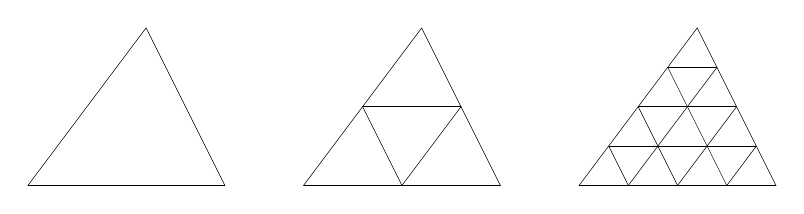
\begin{tikzpicture}
    \tkzDefPoint(-3.5,0){A''}
    \tkzDefPoint(-2,2){B''}
    \tkzDefPoint(-1,0){C''}
    \tkzDrawSegments(A'',B'' B'',C'' A'',C'')

    \tkzDefPoint(0,0){A}
    \tkzDefPoint(1.5,2){B}
    \tkzDefPoint(2.5,0){C}
    \tkzDrawSegments(A,B B,C A,C)

    \tkzDefMidPoint(A,B) \tkzGetPoint{ab}
    \tkzDefLine[orthogonal=through ab](A,B)
    \tkzDefMidPoint(A,C) \tkzGetPoint{ac}
    \tkzDefLine[orthogonal=through ac](A,C)
    \tkzDefMidPoint(B,C) \tkzGetPoint{bc}
    \tkzDefLine[orthogonal=through bc](B,C)
    \tkzDrawSegment(ab,ac)
    \tkzDrawSegment(ab,bc)
    \tkzDrawSegment(ac,bc)

    \tkzDefPoint(3.5,0){A'}
    \tkzDefPoint(5,2){B'}
    \tkzDefPoint(6,0){C'}
    \tkzDrawSegments(A',B' B',C' A',C')
    \tkzDefMidPoint(A',B') \tkzGetPoint{ab'}
    \tkzDefLine[orthogonal=through ab'](A',B')
    \tkzDefMidPoint(A',C') \tkzGetPoint{ac'}
    \tkzDefLine[orthogonal=through ac'](A',C')
    \tkzDefMidPoint(B',C') \tkzGetPoint{bc'}
    \tkzDefLine[orthogonal=through bc'](B',C')
    \tkzDrawSegment(ab',ac')
    \tkzDrawSegment(ab',bc')
    \tkzDrawSegment(ac',bc')

    \tkzDefMidPoint(A',ab') \tkzGetPoint{aab}
    \tkzDefLine[orthogonal=through aab](A',ab')
    \tkzDefMidPoint(A',ac') \tkzGetPoint{aac}
    \tkzDefLine[orthogonal=through aac](A',ac')
    \tkzDefMidPoint(ac',ab') \tkzGetPoint{x}
    \tkzDefLine[orthogonal=through x](ac',ab')
    \tkzDrawSegment(aab,aac)
    \tkzDrawSegment(aab,x)
    \tkzDrawSegment(aac,x)

    \tkzDefMidPoint(B',ab') \tkzGetPoint{abb}
    \tkzDefLine[orthogonal=through abb](B',ab')
    \tkzDefMidPoint(B',bc') \tkzGetPoint{bbc}
    \tkzDefLine[orthogonal=through bbc](B',bc')
    \tkzDefMidPoint(bc',ab') \tkzGetPoint{y}
    \tkzDefLine[orthogonal=through y](bc',ab')
    \tkzDrawSegment(abb,bbc)
    \tkzDrawSegment(abb,y)
    \tkzDrawSegment(bbc,y)

    \tkzDefMidPoint(C',ac') \tkzGetPoint{acc}
    \tkzDefLine[orthogonal=through acc](C',ac')
    \tkzDefMidPoint(C',bc') \tkzGetPoint{bcc}
    \tkzDefLine[orthogonal=through bcc](C',bc')
    \tkzDefMidPoint(bc',ac') \tkzGetPoint{z}
    \tkzDefLine[orthogonal=through z](bc',ac')
    \tkzDrawSegment(acc,bcc)
    \tkzDrawSegment(acc,z)
    \tkzDrawSegment(bcc,z)

    \tkzDefMidPoint(ab',ac') \tkzGetPoint{l}
    \tkzDefLine[orthogonal=through l](ab',ac')
    \tkzDefMidPoint(ab',bc') \tkzGetPoint{m}
    \tkzDefLine[orthogonal=through m](ab',bc')
    \tkzDefMidPoint(ac',bc') \tkzGetPoint{r}
    \tkzDefLine[orthogonal=through r](ac',bc')
    \tkzDrawSegment(l,m)
    \tkzDrawSegment(l,r)
    \tkzDrawSegment(m,r)

    \end{tikzpicture}
    \caption{Illustration of red refinement, starting with a single triangle and two successive refinement steps}
    \label{Fig3}%change all after!!!
    \end{figure}

    Let $T = [x^0, x^1, x^2]$ be the triangle to be refined, and denote $x^{ij}$ by the midpoint of the edge between $x^i$ and $x^j$.\\
    \textbf{Algorithm} Red refinement in 2D \{\\
    $T_1 := [x^0, x^{01}, x^{02}]; \qquad T_2 := [x^{01}, x^{1}, x^{12}];$\\
    $T_3 := [x^{02}, x^{12}, x^2]; \qquad T_4 := [x^{01}, x^{12}, x^{02}];$\\
    \}



    \begin{lemma*}
    Red refinement gives same congruence class in 2-dimension case.
    \end{lemma*}
    \begin{proof}\mbox{}\\
    \begin{figure}
    \centering
    \begin{tikzpicture}[scale=0.8]
    \tkzDefPoint(0,0){A}
    \tkzDefPoint(1.5,2){B}
    \tkzDefPoint(2.5,0){C}
    \tkzDrawSegments(A,B B,C A,C)

    \tkzLabelPoints[above,yshift=0pt](B)
    \tkzLabelPoints[left,yshift=4pt](A)
    \tkzLabelPoints[right,yshift=4pt](C)
    \tkzDefMidPoint(A,B) \tkzGetPoint{X}
    \tkzDefLine[orthogonal=through ab](A,B)
    \tkzDefMidPoint(A,C) \tkzGetPoint{Z}
    \tkzDefLine[orthogonal=through ac](A,C)
    \tkzDefMidPoint(B,C) \tkzGetPoint{Y}
    \tkzDefLine[orthogonal=through bc](B,C)
    \tkzDrawSegment(X,Z)
    \tkzDrawSegment(X,Y)
    \tkzDrawSegment(Z,Y)
    \tkzLabelPoints[above,xshift=-2mm](X)
    \tkzLabelPoints[above,xshift=2mm](Y)
    \tkzLabelPoints[below](Z)
    \end{tikzpicture}
    \caption{Illustration of Uniform Refinement for the Lemma}
    \end{figure}

    Let A, B, C be the vertices of the triangle $T$ and let X, Y, Z be the midpoints of the edge AB, BC and AC. An application of red refinement produces the triangle $T_1 = [A, X, Z]$, $T_2 = [X, B, Y]$, $T_3 = [Z, Y, C]$ and $T_4 = [Y, Z, X]$. Consider the picture above.

    We have line XY parallel to line AC, i.e., $XY \parallel AC$, so $\angle{BXY} = \angle{XAZ}$. Similarily, since $XZ\parallel BC$, we have $\angle{XBY} = \angle{AXZ}$. Since X is the midpoint of line AB, then $|AX| = |BX|$. In short, we have 
    \begin{align*}
    \angle{BXY} = \angle{XAZ},
    \quad
    |BX| = |AX|,
    \quad
    \angle{XBY} = \angle{AXZ}.
    \end{align*}
    Therefore, $\triangle{BXY} \cong \triangle{XAZ}$. Similarily, we can prove the four triangles are congruent to each other, i.e., $\triangle{BXY}\cong\triangle{XAZ}\cong\triangle{YZC} \cong\triangle{ZYX}$, so they are in a same congruent class, which is same as the one of the original triangle $\triangle{BAC}$.
    \end{proof}
    By the lemma above, we know that red refinement applied on a non degenerate simplex in 2 dimension gives one congruent class. Moreover, by Theorem in 3.1, we see that red refinement strategy is stable.
    [This lemma leads to stability]

    \begin{lemma*}
    Red refinement preserves consistency in 2-dimension case.
    \end{lemma*}
    \begin{proof}\mbox{}\\
    This is obvious as how simplicial complex is defined.
    \end{proof}

    \paragraph{Stability and Consistency}\mbox{}\\
    Subdividing a triangle by connecting its midpoint, we obtain four congruent simplices $T_1, T_2, T_3$ and $T_4$. The green refinement, an irregular refinement which connects the refined edge midpoint to its opposite corner, is applied on one refined edge on which we may confront with degenerate simplices. We will never touch and refine such simplices to avoid them from degenerating.

    Clearly, the red refinement strategy is stable since it produces a finite number of triangles congruent to the original simplex. Meanwhile, we preserve consistency by bisecting triangles with one refined edge and never refine them any further. Therefore, we obtain stability and consistency through red and green refinement.

    \paragraph{Vertices and Edges by Red Refinement in 2D}\mbox{}\\
    In Figure 2 above, we see that we obtain four congruent triangles similar to the original large triangle. Lemma 1 below presents relationship between number of triangles and number of times that red refinement is applied.

    \begin{lemma}
    Denote $T_{m}$ as the number of triangles after applying red refinement m times, then,
    \begin{align*}
    T_{m+1} = 4 \cdot T_{m}, \quad T_{m} = 4^m \cdot T_0
    \end{align*}
    \end{lemma}
    \begin{proof}
    Based on Figure 3, we see that we always obtain 4 similar triangles that is same as the original one. In other words, we have $T_{m+1} = 4 \cdot T_{m}$.\\
    To prove $T_{m} = 4^m \cdot T_0$ by induction, we have the base case that $T_1 = 4^1 \cdot T_0$ in Figure 3. Suppose that this is true for $T_{m} = 4^m \cdot T_0$, we need to prove this holds true for $T_{m+1}$.\\
    Since we have $T_{m+1} = 4 \cdot T_{m}$, and by inductive hypothesis, we have
    \begin{align*}
    T_{m+1} = 4 \cdot T_{m} = 4 \cdot (4^m\cdot T_0) = 4^{m+1}\cdot T_0
    \end{align*}
    Therefore, by induction, we proved that $T_{m+1} = 4 \cdot T_{m}$.
    \end{proof}

    \begin{lemma}
    Denote $E_{m}$ as the number of edges of a simplicial complex $\mathcal{T}$ [Or simplex???] obtained by applying red refinement m times, then,
    \begin{align*}
    E_{m+1} = 2 \cdot E_m + 3 \cdot T_m, \quad E_{m} = 2^{m}\cdot E_0 + 3 \cdot2^{m-1}\cdot(2^{m} -1)\cdot T_0
    \end{align*}
    \end{lemma}
    \begin{proof}
    After applying the red refinement one more time, that is m+1 times in total, then we can think like in each smaller triangle in $T_m$, we again have double number of edges by bisecting edges, and obtain number of $T_m$ edges from connecting each midpoints. Therefore, we have $E_{m+1} = 2\cdot E_m + 3\cdot T_m$.\\
    The proof of the latter part can also be done by induction. The base case is obvious by Figure 3, that is $E_1 = 9 = 2^1\cdot 3 + 3\cdot 2^0 \cdot (2^1 - 1)\cdot1 = 2^1\cdot E_0 + 3\cdot2^{1-1}\cdot(2^1 - 1)\cdot T_0$.\\
    Suppose that this holds after applying red refinement m times, i.e., $E_{m} = 2^{m} E_0 + 3 \cdot2^{m-1}\cdot(2^{m} -1)\cdot T_0$. Since $E_{m+1} = 2 \cdot E_m + 3 \cdot T_m$, and by the inductive hypothesis and Lemma 1, we have
    \begin{align*}
    E_{m+1} &= 2 \cdot E_m + 3 \cdot T_m \\
    &= 2(2^{m}\cdot E_0 + 3 \cdot2^{m-1}\cdot(2^{m} -1)\cdot T_0) + 3\cdot 4^m\cdot T_0\\
    &= 2^{m+1}\cdot E_0 + 3\cdot2^m\cdot(2^m - 1)\cdot T_0 + 3\cdot4^m\cdot T_0\\
    &= 2^{m+1}\cdot E_0 + 3\cdot(2^m\cdot(2^m -1 + 2^m))\cdot T_0\\
    &=2^{m+1}\cdot E_0 + 3\cdot2^m\cdot(2^{m+1}-1)\cdot T_0\\
    \end{align*}
    Thus, we finished the proof by induction.
    \end{proof}

    \begin{lemma}
    Denote $V_{m}$ as the number of vertices of a simplicial complex $\mathcal{T}$ [Or simplex???] obtained by applying red refinement m times, then,
    \begin{align*}
    V_{m+1} = V_{m} + E_{m}, \quad V_m = V_0 + (2^m -1)\cdot E_0 + (2^{m-1}\cdot(2^m+3)-2)\cdot T_0
    \end{align*}
    \end{lemma}
    \begin{proof}
    Whenever red refinement is applied, we set a midpoint on each edge as a new vertex. That is, we obtain a same number of new vertices as the number of edges of the simplicial complex before applying the red refinement. After applying the red refinement one more time, the number of new vertices is same as the number of edges of $T_m$, i.e., $E_m$. Then adding together, we have $V_{m+1} = V_m + E_m$.\\
    Suppose that $V_m = V_0 + (2^m -1)\cdot E_0 + (2^{m-1} -1)(2^m -1)\cdot T_0$. Then by Lemma 2, we have
    \begin{align*}
    V_{m+1} &= V_m + E_m\\
    &= V_m + 2^m\cdot E_0 + 3\cdot 2^{m-1}\cdot(2^m-1)\cdot T_0\\
    &= V_0 + \sum_{k=0}^m 2^k E_0 + 3\cdot 2^{k-1}\cdot(2^k-1)\cdot T_0\\
    &= V_0 + \sum_{k=0}^m 2^k E_0 + 3\sum_{k=0}^m 2^{2k-1}\cdot T_0 + 3\sum_{k=0}^m 2^{k-1}\cdot T_0\\
    &= V_0 + (2^{m+1}-1)E_0 + \frac{3}{2}\sum_{k=0}^m 4^k\cdot T_0 + \frac{3}{2}\sum_{k=0}^m 2^k\cdot T_0\\
    &= V_0 + (2^{m+1}-1)E_0 + \frac{3}{2}\cdot\frac{4^{m+1}-1}{3}\cdot T_0 + \frac{3}{2}(2^{m+1}-1)\cdot T_0\\
    &= V_0 + (2^{m+1}-1)E_0 + \frac{4^{m+1}-1 + 3\cdot2^{m+1} -3}{2}\cdot T_0\\
    &= V_0 + (2^{m+1}-1)E_0 + (2^m\cdot(2^{m+1}+3)-2)\cdot T_0
    \end{align*}
    Thus, we finished the proof.
    \end{proof}


    \subsection{3D}

  \section{Bisection}
        \subsection{Bisection Refinement in 2-dimension}
    Another popular refinement strategy is bisection. Basically, we cut a triangle by connecting one vertex, which we choose as the peak, with its opposite edge, which we call refinement edge. Generally, if we apply random bisection with no plan on a triangle, it is likely that we fail to preserve stability and consistency.

    Hence, one important part we need to consider is how to choose the peak for a triangle to preserve the stability and consistency, and one famous method was introduced as the $newest vertex$ bisection. In newest vertex bisection, we create the newest vertex at the middle of the refinement edge after applying the bisection refinement once, and then we regard the newest vertex as the peak for bisection over the resulting two smaller triangles.

    \begin{figure}[h!]
    \centering
      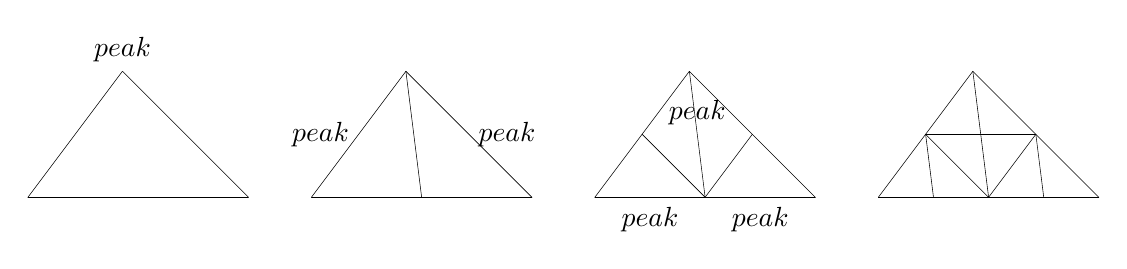
\begin{tikzpicture}[scale=0.8]
      \tkzDefPoint(-6.5,0){A''}
      \tkzDefPoint(-5,2){peak}
      \tkzDefPoint(-3,0){C''}
      \tkzDrawSegments(A'',peak peak,C'' A'',C'')
    %\tkzDrawSegments(A'',B'' B'',C'' A'',C'')
      \tkzLabelPoints[above,yshift=0pt](peak)
    %\tkzDefMidPoint(A'',C'') \tkzGetPoint{new vertex}
    %\tkzLabelPoints[below,yshift=0pt](new vertex)
    %\tkzDefLine[orthogonal=through ac](A,C)
    
    \tkzDefPoint(-2,0){A}
    \tkzDefPoint(-0.5,2){B}
    \tkzDefPoint(1.5,0){C}
    \tkzDrawSegments(A,B B,C A,C)
    \tkzDefMidPoint(A,B) \tkzGetPoint{peak}
    \tkzLabelPoints[left](peak)
    \tkzDefMidPoint(B,C) \tkzGetPoint{peak}
    \tkzLabelPoints[right](peak)
    \tkzDefMidPoint(A,C) \tkzGetPoint{ac}
    \tkzDefLine[orthogonal=through ac](A,C)
    \tkzDrawSegment(B,ac)


    \tkzDefPoint(2.5,0){A'}
    \tkzDefPoint(4,2){B'}
    \tkzDefPoint(6,0){C'}
    \tkzDrawSegments(A',B' B',C' A',C')
    \tkzDefMidPoint(A',B') \tkzGetPoint{ab'}
    \tkzDefLine[orthogonal=through ab'](A',B')
    \tkzDefMidPoint(A',C') \tkzGetPoint{ac'}
    \tkzDefLine[orthogonal=through ac'](A',C')
    \tkzDefMidPoint(B',C') \tkzGetPoint{bc'}
    \tkzDefLine[orthogonal=through bc'](B',C')
    \tkzDrawSegment(B',ac')
    \tkzDrawSegment(ac',ab')
    \tkzDrawSegment(ac',bc')
    \tkzDefMidPoint(B',ac') \tkzGetPoint{peak}
    \tkzLabelPoints[above,yshift=0pt](peak)
    \tkzDefMidPoint(A',ac') \tkzGetPoint{peak}
    \tkzLabelPoints[below](peak)
    \tkzDefMidPoint(C',ac') \tkzGetPoint{peak}    
    \tkzLabelPoints[below](peak)


    \tkzDefPoint(7,0){A'''}
    \tkzDefPoint(8.5,2){B'''}
    \tkzDefPoint(10.5,0){C'''}
    \tkzDrawSegments(A''',B''' B''',C''' A''',C''')
    \tkzDefMidPoint(A''',B''') \tkzGetPoint{ab''}
    \tkzDefLine[orthogonal=through ab''](A''',B''')
    \tkzDefMidPoint(A''',C''') \tkzGetPoint{ac''}
    \tkzDefLine[orthogonal=through ac''](A''',C''')
    \tkzDefMidPoint(B''',C''') \tkzGetPoint{bc''}
    \tkzDefLine[orthogonal=through bc''](B''',C''')
    \tkzDrawSegment(B''',ac'')
    \tkzDrawSegment(ac'',ab'')
    \tkzDrawSegment(ac'',bc'')
    \tkzDefMidPoint(B''',ac'') \tkzGetPoint{x}
    \tkzDefLine[orthogonal=through x](B''',ac'')
    \tkzDefMidPoint(A''',ac'') \tkzGetPoint{y}
    \tkzDefLine[orthogonal=through y](A''',ac'')
    \tkzDefMidPoint(C''',ac'') \tkzGetPoint{z}
    \tkzDefLine[orthogonal=through z](C''',ac'')
    \tkzDrawSegment(ab'',x)
    \tkzDrawSegment(bc'',x)
    \tkzDrawSegment(ab'',y)
    \tkzDrawSegment(bc'',z)
    \end{tikzpicture}
    \caption{Illustration of bisection refinement, starting with a single triangle}
    \label{Fig4}
    \end{figure}







%----------------------------------------------------------------------------------
    \begin{lemma*}
    Bisection refinement gives four congruence classes given one triangle.
    \end{lemma*}
    \begin{proof}
    \begin{figure}[h!]
    \centering
      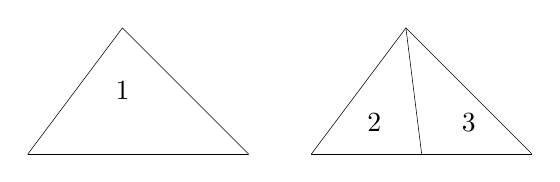
\begin{tikzpicture}[scale=0.8]
      \tkzDefPoint(-6.5,0){A''}
      \tkzDefPoint(-5,2){B''}
      \tkzDefPoint(-3,0){C''}
      \tkzDrawSegments(A'',B'' B'',C'' A'',C'')
      \node (t) at (-5, 1) {{1}};

      \tkzDefPoint(-2,0){A}
      \tkzDefPoint(-0.5,2){B}
      \tkzDefPoint(1.5,0){C}
      \tkzDrawSegments(A,B B,C A,C)
      \tkzDefMidPoint(A,C) \tkzGetPoint{ac}
      \tkzDefLine[orthogonal=through ac](A,C)
      \tkzDrawSegment(B,ac)
      \node (t') at (-1, 0.5) {{2}};
      \node (t'') at (0.5, 0.5) {{3}};
      \end{tikzpicture}
    \caption{Stage 1: Original triangle(left); Stage 2: Applied the newest vertex bisection once(right)}
    \label{fig5: sub1}
    \end{figure}

    Observing Figure 5, we have a triangle at the beginning, say it's in congruency class 1. After applying the newest vertex bisection refinement once, we obtain two smaller pieces of triangles as in the second picture in Figure 5. Say one of them is in congruency class 2, and another one is in congruency class 3. Further applying the newest vertex bisection refinement, we have the figures below.

    \begin{figure}[h!]
    \centering
      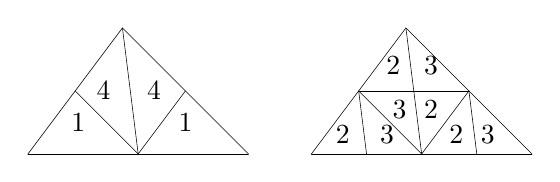
\begin{tikzpicture}[scale=0.8]
      \tkzDefPoint(2.5,0){A'}
      \tkzDefPoint(4,2){B'}
      \tkzDefPoint(6,0){C'}
      \tkzDrawSegments(A',B' B',C' A',C')
      \tkzDefMidPoint(A',B') \tkzGetPoint{ab'}
      \tkzDefLine[orthogonal=through ab'](A',B')
      \tkzDefMidPoint(A',C') \tkzGetPoint{ac'}
      \tkzDefLine[orthogonal=through ac'](A',C')
      \tkzDefMidPoint(B',C') \tkzGetPoint{bc'}
      \tkzDefLine[orthogonal=through bc'](B',C')
      \tkzDrawSegment(B',ac')
      \tkzDrawSegment(ac',ab')
      \tkzDrawSegment(ac',bc')
      \node (t''') at (3.7, 1) {{4}};
      \node (t''') at (4.5, 1) {{4}};
      \node (t) at (3.3, 0.5) {{1}};
      \node (t) at (5, 0.5) {{1}};

      \tkzDefPoint(7,0){A'''}
      \tkzDefPoint(8.5,2){B'''}
      \tkzDefPoint(10.5,0){C'''}
      \tkzDrawSegments(A''',B''' B''',C''' A''',C''')
      \tkzDefMidPoint(A''',B''') \tkzGetPoint{ab''}
      \tkzDefLine[orthogonal=through ab''](A''',B''')
      \tkzDefMidPoint(A''',C''') \tkzGetPoint{ac''}
      \tkzDefLine[orthogonal=through ac''](A''',C''')
      \tkzDefMidPoint(B''',C''') \tkzGetPoint{bc''}
      \tkzDefLine[orthogonal=through bc''](B''',C''')
      \tkzDrawSegment(B''',ac'')
      \tkzDrawSegment(ac'',ab'')
      \tkzDrawSegment(ac'',bc'')
      \tkzDefMidPoint(B''',ac'') \tkzGetPoint{x}
      \tkzDefLine[orthogonal=through x](B''',ac'')
      \tkzDefMidPoint(A''',ac'') \tkzGetPoint{y}
      \tkzDefLine[orthogonal=through y](A''',ac'')
      \tkzDefMidPoint(C''',ac'') \tkzGetPoint{z}
      \tkzDefLine[orthogonal=through z](C''',ac'')
      \tkzDrawSegment(ab'',x)
      \tkzDrawSegment(bc'',x)
      \tkzDrawSegment(ab'',y)
      \tkzDrawSegment(bc'',z)
      \node (t') at (7.5, 0.3) {{2}};
      \node (t'') at (8.2, 0.3) {{3}};
      \node (t'') at (8.4, 0.7) {{3}};
      \node (t') at (8.3, 1.4) {{2}};
      \node (t'') at (8.9, 1.4) {{3}};
      \node (t') at (8.9, 0.7) {{2}};
      \node (t') at (9.3, 0.3) {{2}};
      \node (t'') at (9.8, 0.3) {{3}};
      \end{tikzpicture}
    \caption{Stage 3: Applied the newest vertex bisection twice(left); Stage 4: Applied the newest vertex bisection three times(right)}
    \label{fig5: sub2}
    \end{figure}

    \begin{claim}
    The left and right bottom triangles in Stage 3 are congruent to the original triangle in Stage 1, and they are in the congruency class 1. Moreover, the other two triangles left are congruent and in congruency class 4.
    \end{claim}
    \begin{proof}\mbox{}\\
    \begin{minipage}[c]{5cm}
    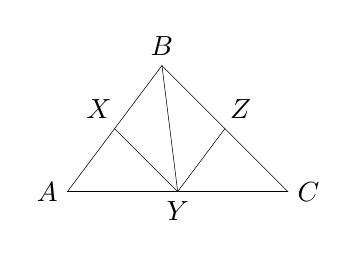
\begin{tikzpicture}[scale=0.8]
    \tkzDefPoint(2.5,0){A}
    \tkzDefPoint(4,2){B}
    \tkzDefPoint(6,0){C}
    \tkzDrawSegments(A,B B,C A,C)
    \tkzLabelPoints[left](A)
    \tkzLabelPoints[above](B)
    \tkzLabelPoints[right](C)
    \tkzDefMidPoint(A,B) \tkzGetPoint{X}
    \tkzDefLine[orthogonal=through X](A,B)
    \tkzDefMidPoint(A,C) \tkzGetPoint{Y}
    \tkzDefLine[orthogonal=through Y](A,C)
    \tkzDefMidPoint(B,C) \tkzGetPoint{Z}
    \tkzDefLine[orthogonal=through Z](B,C)
    \tkzDrawSegment(B,Y)
    \tkzDrawSegment(Y,X)
    \tkzDrawSegment(Y,Z)
    \tkzLabelPoints[above, xshift=-2mm](X)
    \tkzLabelPoints[above, xshift=2mm](Z)
    \tkzLabelPoints[below,yshift=0pt](Y)
    \end{tikzpicture}
    \end{minipage}
    \begin{minipage}[c]{\textwidth-6cm}
    Let A, B, C be the vertices of the triangle $T$ and let X, Y, Z be the midpoints of the edge AB, AC and BC. An application of the newest vertex bisection refinement produces the triangle $\triangle{AXY}, \triangle{XBY}, \triangle{ZBY}$ and $\triangle{YZC}$. Consider the picture on the left.
    \end{minipage}
    Since X, Y, Z be the midpoints of the edge AB, AC and BC, we have $XY\parallel BC, ZY\parallel AB$, and AX = BX, BZ = CZ, and AY = CY. Since $XY\parallel BC$, $\angle{AXY} = \angle{ABC}, \angle{XYB} = \angle{ZBY}$. Similarly, since $ZY\parallel AB$, $\angle{YZC} = \angle{ABC}, \angle{XBY} = \angle{ZYB}$
    \begin{align*}
    \angle{XYB} &= \angle{ZBY}\\
    |BY| &= |BY|\\
    \angle{XBY} &= \angle{ZYB}
    \end{align*}
    Therefore, we have $\triangle{XBY} \cong \triangle{ZYB}$, and we mark them in the congruency class 4. This further gives us $|AX| = |BX| = |YZ|$, and $|ZC| = |BZ| = |XY|$.
    \begin{align*}
    |AX| &= |YZ|\\
    \angle{AXY} &= \angle{ABC} = {YZC}\\
    |XY| &= |ZC|
    \end{align*}
    Therefore, we have $\triangle{AXY} \cong \triangle{YZC}$. It's clear that $\triangle{AXY}$ and $\triangle{YZC}$ are similar to $\triangle{ABC}$ as all their angles are the same. Thus, we finished the proof of claim 1.

    \end{proof}%end proof of claim 1

    \begin{claim}
    Triangles with same number in Stage 4 in a same congruency class marked by the number.
    \end{claim}
    \begin{proof}
    Note [NEED TO BE UPDATED]
    \end{proof}
    Notice that in Stage 3, we see triangles in congruency class 1 again, so we can tell further applying the newest vertex bisection refinement will lead to the same process as what we have for Stage 1. Similarly, further applying the newest vertex bisection refinement over triangles in congruency class 4, 2 and 3 are already explored in Stage 3 and 4. Therefore, we actually obtain 4 congruency classes only.
    \end{proof}
    This means that we never have triangles degenerating when applying the newest vertex bisection refinement, because the number of congruence classes is four, which is finite, and by theorem proved in 3.1, we see that the newest vertex bisection refinement strategy is stable.

    As we explain in section 3, a good refinement strategy should preserve both stability and consistency. To further explore consistency...[NEED TO BE UPDATED]
    \begin{lemma*}
    Question: consistency? Compatibility chain[YES]
    \end{lemma*}

  \newpage
  \bibliographystyle{abbrvnat}
  \bibliography{Bib}
    
  %\subsection{}
\end{document}